\documentclass[aspectratio=169]{beamer}

\usetheme{default}
\usecolortheme{default}
\setbeamertemplate{navigation symbols}{}
\setbeamertemplate{footline}[frame number]
\setbeamercolor{title}{fg=black}
\setbeamercolor{frametitle}{fg=black}
\setbeamerfont{frametitle}{series=\bfseries}

\usepackage[T1]{fontenc}
\usepackage[utf8]{inputenc}
\usepackage[brazil]{babel}
\usepackage{graphicx}
\usepackage{amsmath}
\usepackage{booktabs}
\usepackage{array}

\title{CERISE — Dois Trabalhos, Uma Base Comum}
\subtitle{LARS 2026 (alocação de tarefas via RL) e LAFusion 2026 (fusão sensorial via EKF)}
\author{Yan Santos Leite}
\institute{Orientador: Prof. Alisson Assis Cardoso \\ Escola de Engenharia Elétrica, Mecânica e de Computação (EMC) — UFG \\ Fundação de Amparo à Pesquisa do Estado de Goiás (FAPEG)}
\date{16 de agosto de 2026}

\begin{document}

% ============================================================
\begin{frame}
\titlepage
\end{frame}

% ============================================================
\begin{frame}{Roteiro}
Esta apresentação cobre a trajetória completa de dois trabalhos que compartilham a mesma base de código e a mesma plataforma física (três TurtleBot3 no CERISE), mas respondem a perguntas de pesquisa diferentes.

\vspace{0.5cm}
\begin{enumerate}
\item \textbf{LARS 2026} — da concepção à submissão (06/08): um agente de RL supera a heurística gulosa na alocação de tarefas? Arquitetura, resultado, diagnóstico causal, fechamento.
\item \textbf{LAFusion 2026} — da concepção ao estado atual (16/08): um EKF de fusão sensorial melhora a localização sob observação visual esparsa? Arquitetura, validação, resultado, achado central.
\item \textbf{Conclusão} — o que cada trabalho contribui e os próximos passos concretos de cada um.
\end{enumerate}

\vspace{0.3cm}
\small Os dois papers reaproveitam a mesma bateria de testes estatísticos (\texttt{stats\_tests.py}: Wilcoxon signed-rank, Cliff's $\delta$, IC bootstrap) — não são iniciativas isoladas, mas duas perguntas feitas sobre a mesma infraestrutura experimental.
\end{frame}

% ============================================================
\begin{frame}{Visão geral dos dois trabalhos}
\begin{center}
\renewcommand{\arraystretch}{1.6}
\begin{tabular}{p{3.3cm}p{4.6cm}p{4.6cm}}
\toprule
 & \textbf{LARS 2026} & \textbf{LAFusion 2026} \\
\midrule
Pergunta & RL supera a heurística gulosa na alocação de tarefas? & EKF melhora a localização sob cobertura visual esparsa? \\
Método & PPO (Stable-Baselines3) & Extended Kalman Filter por robô \\
Plataforma & 3 TurtleBot3, ROS2/Gazebo & 3 TurtleBot3, ROS2/Gazebo \\
Estado & Submetido no EasyChair em 06/08 & 8 páginas prontas, prazo 04/09 \\
\bottomrule
\end{tabular}
\end{center}
\vspace{0.3cm}
Os dois trabalhos compartilham a câmera overhead + detector YOLOv8n como fonte de posição, mas usam esse dado de formas opostas: o LARS o consome diretamente como estado observado pelo agente; o LAFusion pergunta o que fazer quando esse dado \emph{nem sempre está disponível}.
\end{frame}

% ============================================================
\section{LARS 2026}

\begin{frame}{LARS — Motivação}
\textbf{O problema.} Alocação de tarefas multi-robô (MRTA) é resolvida na prática por heurísticas gulosas: atribuem a tarefa ao robô livre mais próximo, sem olhar para demandas futuras. São rápidas e respeitam restrições operacionais por construção (nunca escolhem um robô ocupado), mas são míopes — não veem que o robô mais próximo agora pode ser o mais útil daqui a pouco.

\vspace{0.3cm}
\textbf{Por que RL.} Uma política aprendida pode, em princípio, trocar uma atribuição localmente subótima por um resultado melhor no conjunto do episódio — é exatamente essa miopia que o RL promete corrigir.

\vspace{0.3cm}
\textbf{Hipótese testada.} Uma política PPO com antecipação de duas demandas futuras supera a heurística \emph{nearest-free} em tempo de resposta.
\end{frame}

% ============================================================
\begin{frame}{LARS — Arquitetura e pipeline}
\textbf{Pipeline conceitual:}
\begin{center}
Câmera overhead $\rightarrow$ YOLOv8n $\rightarrow$ \texttt{/robot\_detections} $\rightarrow$ AllocationEnv $\rightarrow$ Política PPO $\rightarrow$ Nav2 $\rightarrow$ TurtleBot3
\end{center}

\vspace{0.3cm}
\textbf{Módulos reais do código:}
\begin{itemize}
\item \texttt{yolo\_detector.py} — nó ROS2 que publica a posição estimada de cada robô a partir da câmera overhead.
\item \texttt{rl/allocation\_env.py} — ambiente Gymnasium \emph{analítico} (sem ROS/Gazebo): cada \texttt{step()} é aritmética pura sobre um modelo de navegação, o que permite treinar 500 mil timesteps em minutos em vez de dias.
\item \texttt{rl\_task\_allocator.py} — nó ROS2 de inferência, que carrega a política treinada no ambiente analítico e a aplica sobre posições reais do YOLO.
\item \texttt{task\_allocator.py} — a heurística \emph{nearest-free}, usada como baseline.
\end{itemize}

\vspace{0.2cm}
\small O treino roda inteiramente no ambiente analítico; o Gazebo é reservado para validação final de ponta a ponta, não para treino — treinar direto no simulador físico custaria ordens de magnitude mais tempo pelo mesmo motivo que qualquer simulação física é mais lenta que aritmética vetorizada.
\end{frame}

% ============================================================
\begin{frame}{LARS — Detecção YOLO: verdade vs. predição}
\begin{columns}[T]
\begin{column}{0.42\textwidth}
\centering
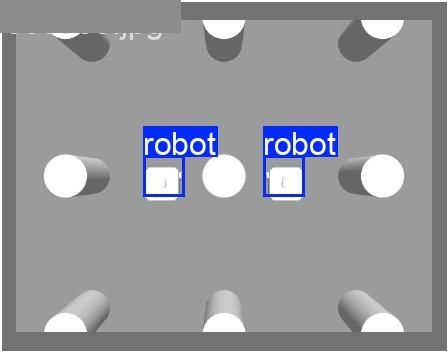
\includegraphics[height=3.1cm]{../paper_lars/en/fig_yolo_labels_crop.jpg}\\
\scriptsize Verdade terrestre
\vspace{0.1cm}

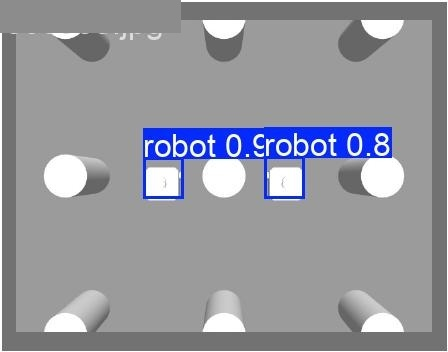
\includegraphics[height=3.1cm]{../paper_lars/en/fig_yolo_pred_crop.jpg}\\
\scriptsize Predição do detector
\end{column}
\begin{column}{0.58\textwidth}
\small Anotação de verdade terrestre vs. predição do detector, mesma cena do conjunto de validação, um a três robôs simultaneamente visíveis.

\vspace{0.2cm}
\small \emph{Por que esta figura importa:} o mAP@0,5=0,995 e o erro de 4,7 cm do próximo slide são médias agregadas — não mostram \emph{como} o detector erra. Esta comparação qualitativa é a evidência de que o erro reportado é bem comportado (caixa acompanha o robô de forma consistente, mesmo com múltiplos robôs próximos) e não um artefato de outliers escondidos pela média.
\end{column}
\end{columns}
\end{frame}

% ============================================================
\begin{frame}{LARS — Gêmeo digital: evolução da precisão}
\begin{columns}
\begin{column}{0.5\textwidth}
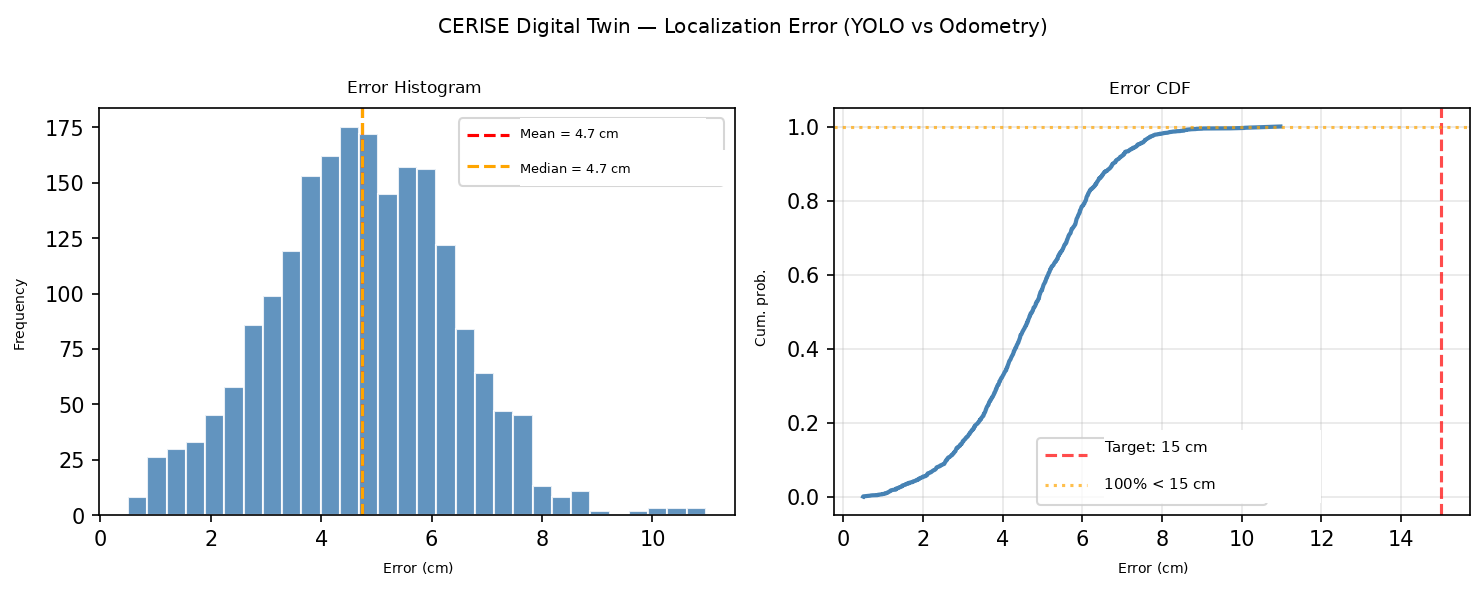
\includegraphics[width=\textwidth]{../paper_lars/en/fig_digitaltwin.png}
\end{column}
\begin{column}{0.5\textwidth}
\textbf{Modelo:} YOLOv8n, 375 frames anotados manualmente.

\vspace{0.2cm}
\begin{tabular}{ll}
mAP@0.5 & \textbf{0,995} \\
Erro estático (8 poses) & 1,24 cm \\
Erro dinâmico (rastreio) & \textbf{4,7 cm} \\
Detecções $<$15 cm & 100\% \\
\end{tabular}

\vspace{0.3cm}
\small O salto de 1,24 cm para 4,7 cm entre o benchmark estático e o rastreamento contínuo é esperado — motion blur e latência de detecção-para-pose em movimento, não uma limitação do detector. É o erro de 4,7 cm, não o estático, que alimenta todos os experimentos seguintes.
\end{column}
\end{columns}
\end{frame}

% ============================================================
\begin{frame}{LARS — Formulação do MDP}
\textbf{Estado (21 dimensões):} para $N=3$ robôs, $3N+4+4\times2=21$ — posição $(x,y)$ e tempo até ficar livre de cada robô, origem/destino da demanda atual, e origem/destino das \textbf{2 próximas demandas} já visíveis na fila.

\vspace{0.2cm}
\small \emph{Por quê a antecipação:} sem ver as próximas demandas, a política não tem como decidir "segurar" um robô livre para uma tarefa melhor que está a caminho — é essa antecipação, e só ela, que poderia justificar vencer a heurística míope.

\vspace{0.3cm}
\textbf{Ação:} escolha discreta de qual dos $N$ robôs atende a demanda atual.

\vspace{0.3cm}
\textbf{Recompensa:} $r = -(t_{espera} + t_{viagem})$ — o \emph{tempo de resposta} completo, não só o tempo de viagem.

\vspace{0.2cm}
\small \emph{Por quê essa correção importa:} a formulação original penalizava só o tempo de viagem até a demanda, ignorando quanto tempo o robô escolhido ainda levaria para ficar livre. Sob essa formulação anterior, um robô ocupado-mas-próximo podia parecer tão bom quanto um livre-mas-distante — a fila nunca era penalizada, e a política enviesava para robôs livres mesmo quando distantes. Foi um bug de causa-raiz corrigido antes do primeiro resultado válido, não um ajuste de sintonia fina.
\end{frame}

% ============================================================
\begin{frame}{LARS — Curva de aprendizado}
\centering
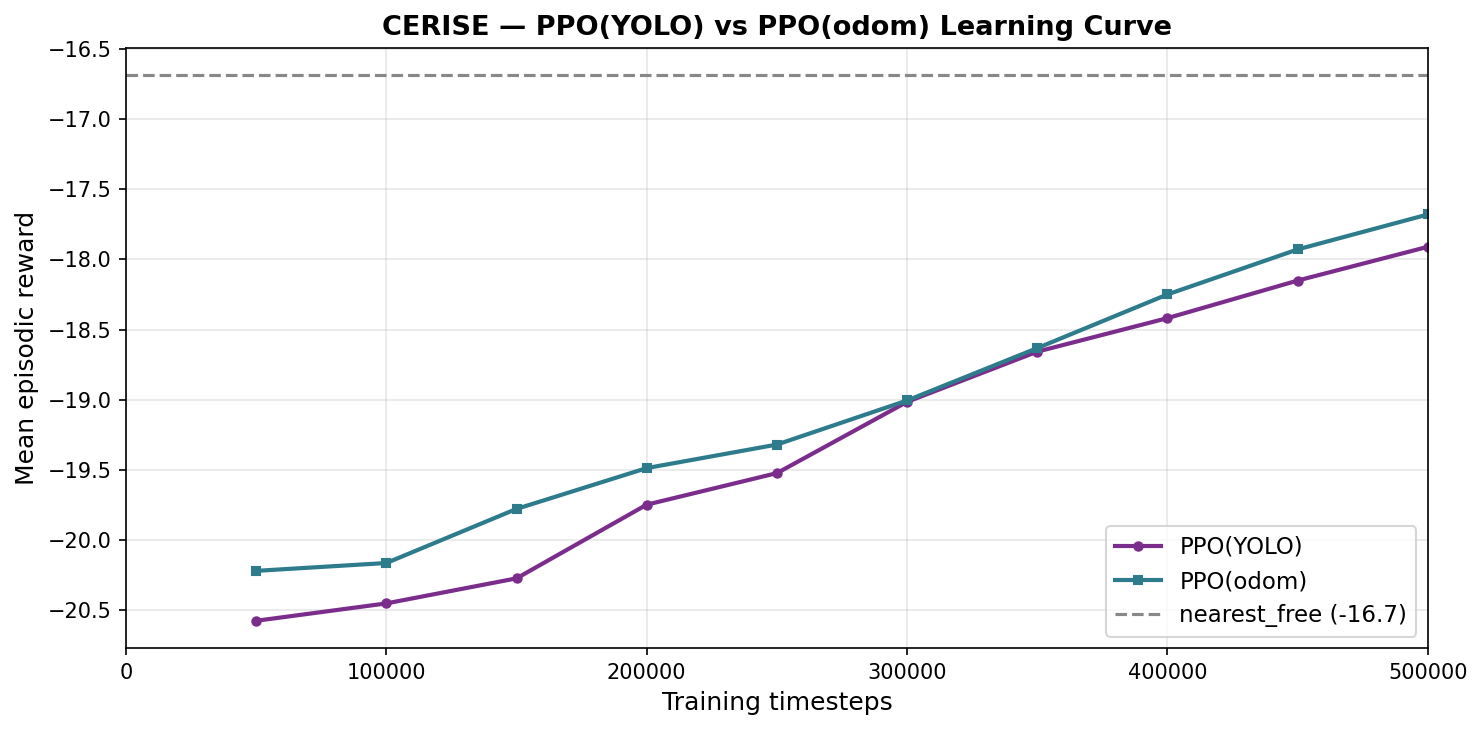
\includegraphics[height=4.6cm]{../paper_lars/en/fig_learning.png}

\vspace{0.15cm}
\small Recompensa média por episódio ao longo de 500 mil timesteps, PPO(YOLO) e PPO(odom), com a linha de referência do guloso ($-16{,}7$).

\vspace{0.1cm}
\scriptsize \emph{Por que esta figura importa:} confirma, antes de qualquer teste estatístico, que o PPO de fato aprendeu ($\sim{-21}\to\sim{-17{,}7}$) — descarta a hipótese trivial de que o resultado negativo dos slides seguintes se deve a um agente que não treinou. Mostra também que \textbf{nenhuma das duas variantes cruza a linha do guloso}, e que PPO(odom) converge ligeiramente mais rápido que PPO(YOLO) — evidência direta de que o ruído do gêmeo digital (4,7 cm) é efeito de segunda ordem, não a causa do gap.
\end{frame}

% ============================================================
\begin{frame}{LARS — Testes e protocolo experimental}
\textbf{Treino:} PPO via Stable-Baselines3, hiperparâmetros \emph{padrão da biblioteca} (taxa de aprendizado $3\times10^{-4}$, $\gamma=0,99$, 8 ambientes paralelos, seed 42), 500 mil timesteps ($\sim$2h CPU).

\vspace{0.2cm}
\small \emph{Por quê hiperparâmetros padrão:} o objetivo do experimento é isolar o efeito da fonte de observação (YOLO vs. odometria) e do \emph{action masking}, não encontrar o teto de desempenho do PPO por meio de tuning — usar os defaults deixa claro que o resultado concerne ao PPO como comumente aplicado, e essa é uma limitação assumida explicitamente no paper, não escondida.

\vspace{0.3cm}
\textbf{Comparação estatística:} 1000 episódios pareados (mesma semente e sequência de demandas entre políticas), \textbf{Wilcoxon signed-rank} para significância, \textbf{Cliff's $\delta$} para tamanho de efeito, IC 95\% bootstrap.

\vspace{0.2cm}
\small \emph{Por quê pareamento:} a variância entre sementes aleatórias, isolada, já produz diferenças estatisticamente significativas em RL profundo — comparar médias sem teste pareado mediria ruído de treino, não a diferença real entre políticas.

\vspace{0.3cm}
\textbf{Robustez sob carga:} varredura de 6 regimes de intervalo entre demandas, de 30s a 10s, 500 episódios por ponto.
\end{frame}

% ============================================================
\begin{frame}{LARS — Primeiro resultado: achado negativo}
\begin{table}
\small
\begin{tabular}{lcccc}
\toprule
\textbf{Política} & \textbf{Resp. média} & \textbf{p95} & \textbf{Custo/ep.} & \textbf{Desbal.} \\
\midrule
Nearest-free & \textbf{17,86 s} & \textbf{27,77 s} & \textbf{357,18 s} & 0,149 \\
PPO (YOLO) & 20,01 s & 29,46 s & 400,20 s & \textbf{0,135} \\
PPO (odom) & 19,83 s & 29,37 s & 396,69 s & \textbf{0,135} \\
\bottomrule
\end{tabular}
\caption{\small Carga moderada (12s entre demandas), 1000 episódios pareados. Wilcoxon $p<0{,}001$ em ambas as comparações contra nearest-free.}
\end{table}

\vspace{0.2cm}
Contra a hipótese, \textbf{o guloso vence} — tempo de resposta médio cerca de \textbf{12\% pior} para o PPO. A diferença entre PPO(YOLO) e PPO(odom) é pequena frente à distância de ambos ao guloso: o ruído de 4,7 cm do gêmeo digital é um efeito de segunda ordem, não a causa do resultado.

\vspace{0.2cm}
\small \textbf{Enquadramento:} um resultado negativo bem caracterizado — testado e explicado — é mais informativo do que uma alegação positiva não testada. É essa caracterização, não a vitória do método proposto, que constitui a contribuição científica aqui.
\end{frame}

% ============================================================
\begin{frame}{LARS — Distribuição completa do tempo de resposta}
\centering
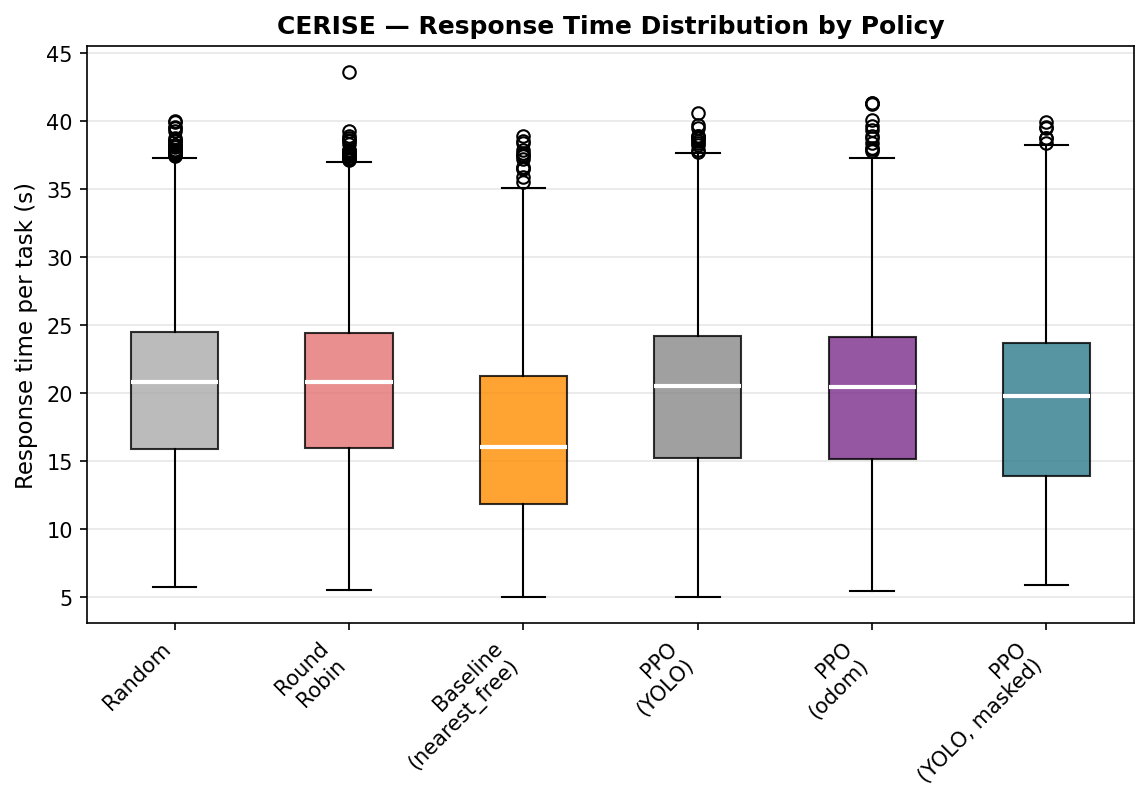
\includegraphics[height=4.8cm]{../paper_lars/en/fig_boxplot.png}

\vspace{0.15cm}
\scriptsize \emph{Por que esta figura importa:} a tabela anterior mostra só médias e p95 — não revela \textbf{onde} na distribuição o PPO perde. Este boxplot mostra que a razão p95/média é comparável entre políticas ($\approx$1,47--1,56) e, de fato, ligeiramente menor para o PPO. Isso descarta uma explicação alternativa plausível (PPO pior só por causa de uma cauda de episódios catastróficos) — a desvantagem vem de um deslocamento de toda a distribuição de tempo de resposta, não de eventos raros.
\end{frame}

% ============================================================
\begin{frame}{LARS — Robustez sob carga}
\centering
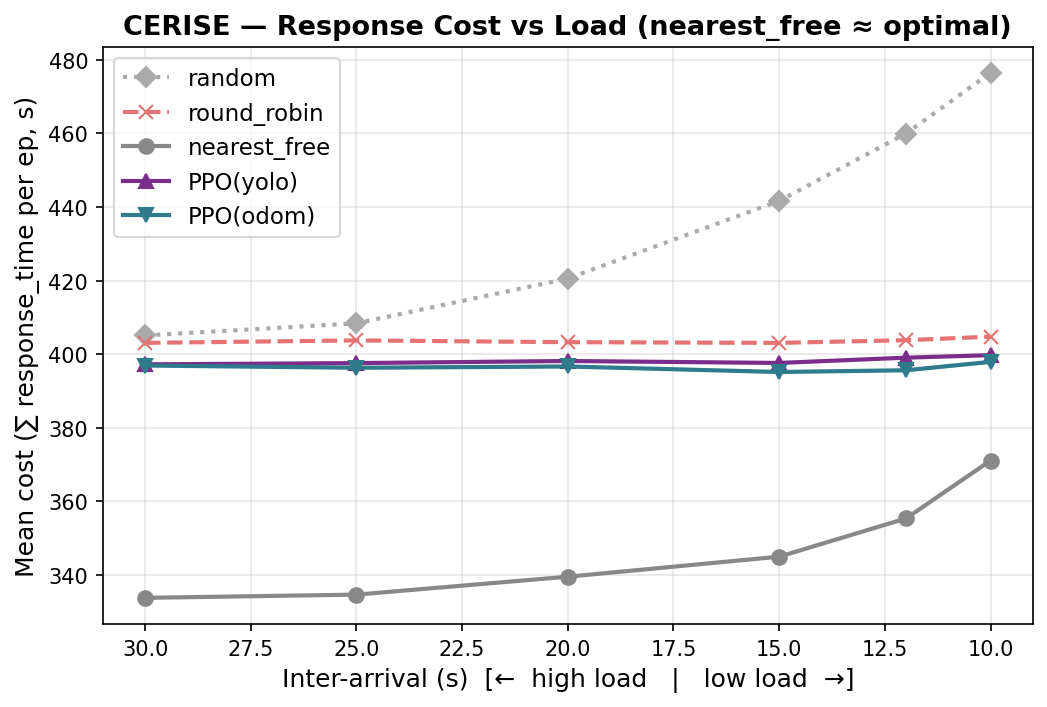
\includegraphics[height=4.4cm]{../paper_lars/en/fig_load.png}

\vspace{0.1cm}
\scriptsize Tempo de resposta em função do intervalo entre demandas (30s a 10s), nearest-free e PPO(YOLO): a desvantagem do PPO \textbf{encolhe} de +19,0\% (carga baixa) para +7,7\% (carga alta), embora o guloso permaneça mais rápido em todo o intervalo testado.

\vspace{0.08cm}
\scriptsize \emph{Por que esta figura importa:} responde a "o resultado é só válido na carga testada?" — o custo do PPO fica quase plano (397--400s) entre regimes, enquanto o do guloso cresce sob carga alta. Sustenta a leitura de que, se existe um ponto de cruzamento onde o PPO supera o guloso, ele está fora do intervalo testado (cargas mais altas ou frotas maiores), não dentro dele.
\end{frame}

% ============================================================
\begin{frame}{LARS — Diagnóstico causal: por que o PPO perde?}
Três explicações foram investigadas antes de qualquer teste:

\begin{itemize}
\item \textbf{Restrição suave vs. rígida.} O guloso nunca escolhe um robô ocupado — a restrição está embutida no próprio algoritmo. O PPO só aprende a evitar isso indiretamente via penalidade no reward, e ainda assim erra em \textbf{4,2\%} das decisões contra \textbf{0,3\%} do guloso ($\sim$13$\times$ mais) — o maior contribuinte isolado encontrado.
\item \textbf{Espaço de ação pequeno.} Com $N=3$, cada decisão tem no máximo três alternativas, limitando qualquer vantagem que a antecipação poderia explorar.
\item \textbf{Orçamento de treino.} 500 mil passos mostraram aprendizado claro, mas não convergência — embora o custo do PPO fique quase constante entre regimes de carga (397–400s) enquanto o do guloso cresce sob carga alta, sugerindo que o platô não é puramente um artefato de orçamento.
\end{itemize}

\vspace{0.2cm}
\small \emph{Por quê testar a restrição suave primeiro:} era a explicação mais barata de testar causalmente (não exige mudar arquitetura nem orçamento) e a mais plausível a priori, dado o fator de 13$\times$ no \texttt{invalid\_rate}.
\end{frame}

% ============================================================
\begin{frame}{LARS — Teste causal: \textit{action masking}}
\textbf{O teste.} Treinamos PPO(YOLO, masked): idêntico ao PPO(YOLO), mas a distribuição de ação é restrita a cada passo aos robôs livres — via \emph{action masking} (MaskablePPO, sb3-contrib), mesmos hiperparâmetros e orçamento de treino.

\vspace{0.3cm}
\begin{tabular}{lcc}
\toprule
 & \textbf{Sem masking} & \textbf{Com masking} \\
\midrule
Taxa de ação inválida & 4,2\% & \textbf{0,0\%} \\
Gap de tempo de resposta vs. guloso & $\sim$12\% & $\sim$11\% \\
Cliff's $\delta$ vs. guloso & 0,703 & 0,636 \\
\bottomrule
\end{tabular}

\vspace{0.3cm}
\textbf{Resultado: a hipótese causal é refutada.} O masking cumpre seu objetivo estrutural — zera a taxa de ação inválida — mas o gap de tempo de resposta melhora só $\sim$1 ponto percentual. A restrição suave não era a causa dominante do gap.

\vspace{0.2cm}
\small \emph{Implicação:} o peso volta para o espaço de ação pequeno e o orçamento de treino. Uma hipótese adicional emerge: ao impedir a política de sequer considerar robôs ocupados, o masking também remove o sinal de aprendizado sobre a consequência dessa escolha — pode reduzir a diversidade de exploração sem trazer, em troca, vantagem de antecipação.
\end{frame}

% ============================================================
\begin{frame}{LARS — Limitações assumidas explicitamente}
O resultado é delimitado por quatro escolhas, reconhecidas no próprio paper:

\begin{enumerate}
\item \textbf{Hiperparâmetros padrão do PPO} — o resultado concerne ao PPO como comumente aplicado, não ao teto do RL para este problema; uma política ajustada pode fechar o gap.
\item \textbf{$N=3$ robôs} — espaço de ação pequeno, e o próprio diagnóstico aponta isso como fator dominante; o achado não deve ser extrapolado para frotas grandes.
\item \textbf{Sem validação em hardware físico} — a política treina no ambiente analítico e é validada de ponta a ponta no Gazebo, mas a transferência sim-to-real permanece não testada.
\item \textbf{500 mil timesteps sem convergência} — houve aprendizado, não convergência.
\end{enumerate}

\vspace{0.3cm}
\small Cada uma dessas quatro limitações é um alvo direto de trabalho futuro — não pontos cegos descobertos depois, mas escopo delimitado desde a escrita do paper.
\end{frame}

% ============================================================
\begin{frame}{LARS — Fechamento: revisão de literatura e submissão}
\textbf{Por que uma revisão sistemática:} para posicionar corretamente um resultado negativo contra o estado da arte, era preciso primeiro mapear esse estado da arte com rigor — sem isso, "o RL não venceu" não se sustenta como contribuição, pode só parecer uma tentativa malfeita.

\vspace{0.3cm}
\textbf{Revisão de literatura:} 330 estudos triados (Scopus, IEEE, arXiv, ACM) $\rightarrow$ \textbf{117 aceitos / 213 rejeitados}, 122 com extração de dados completa.

\vspace{0.3cm}
\textbf{Submissão:} 06/08/2026, 03:17 UTC, EasyChair (LARS 2026), dentro do prazo. Notificação de aceite prevista para \textbf{15/09/2026}.

\vspace{0.3cm}
\textbf{Título final:} \emph{"Causal Diagnosis of Reinforcement Learning Performance in Vision-Based Multi-Robot Task Allocation with a Digital Twin"} — o título já declara o método (diagnóstico causal), não uma alegação de vitória do RL.
\end{frame}

% ============================================================
\begin{frame}{Transição: por que um segundo paper?}
O LARS usa a posição do YOLO como estado observado pelo agente — mas nunca pergunta \emph{o que fazer quando essa detecção não está disponível}. Em produção, isso é tratado por um \textbf{fallback discreto}: confiar na detecção quando associada, na odometria caso contrário.

\vspace{0.3cm}
\textbf{O gap técnico:} um fallback discreto descarta informação — não há correção parcial de detecções de baixa confiança, não há propagação formal de incerteza, e não há comportamento principiado durante longos períodos sem detecção visual.

\vspace{0.3cm}
\textbf{A pergunta do LAFusion:} um Extended Kalman Filter, que funde as duas fontes de forma probabilística em vez de escolher uma ou outra, melhora a localização sob a cobertura visual esparsa que uma câmera fixa realmente produz?
\end{frame}

% ============================================================
\section{LAFusion 2026}

\begin{frame}{LAFusion — Arquitetura e pipeline}
\textbf{Pipeline conceitual:}
\begin{center}
Câmera overhead fixa $\rightarrow$ YOLOv8n $\rightarrow$ Associação (Mahalanobis) $\rightarrow$ EKF por robô $\rightarrow$ pose fundida
\end{center}

\vspace{0.3cm}
\textbf{Módulos reais do código:}
\begin{itemize}
\item \texttt{ekf\_fusion\_node.py} — nó ROS2 de produção: um EKF independente por robô, predição via odometria, correção via detecção YOLO.
\item \texttt{association.py} — gating de Mahalanobis compartilhado entre o EKF e o nó de avaliação offline.
\item \texttt{projection.py} — projeção pixel$\leftrightarrow$mundo, com duas implementações confirmadas geometricamente equivalentes (heurística por FOV e via intrínsecos calibrados).
\end{itemize}

\vspace{0.3cm}
\textbf{Por que EKF, e não UKF ou filtro de partículas:} o modelo de observação da câmera é quase linear (projeção pinhole numa cena essencialmente planar) — o ganho de um UKF, que mira não-linearidade do modelo de observação, seria marginal aqui. O problema central deste trabalho é a \emph{taxa} de observação, não a forma do modelo, e nenhuma dessas alternativas resolve isso (detalhado dois slides à frente).
\end{frame}

% ============================================================
\begin{frame}{LAFusion — Design do EKF}
\textbf{Estado:} $x_k = [p_x, p_y, \theta]^\top$ por robô. A predição integra o \emph{delta} de leituras consecutivas de odometria sobre o estado atual — não o valor absoluto, que descartaria correções visuais anteriores.

\vspace{0.3cm}
\textbf{Hiperparâmetros e sua origem:}
\begin{itemize}
\item $Q = \text{diag}(0{,}5,\ 0{,}5,\ 0{,}25)$ — calibrado empiricamente contra dados reais (varredura de $10^{-6}$ a $1{,}0$; ganho cresce monotonicamente até saturar em $Q\geq0{,}5$).
\item Teto de covariância $\text{clip}(P, -\infty, 0{,}05)$ — \emph{sem} ele, $P$ crescia sem limite em intervalos longos sem correção (traço observado $\approx$85 contra esperado $\approx$0,5), quebrando o gating de Mahalanobis ao alargar a região de aceitação até um robô "roubar" a detecção do vizinho.
\item Limiar de gating $d^2 \leq 9{,}21$ — valor padrão do teste $\chi^2$ com 2 graus de liberdade a 99\% de confiança, não um número ajustado ad hoc.
\end{itemize}

\vspace{0.15cm}
\scriptsize \emph{Por quê o teto de covariância existe:} mantém a associação estável, não torna a estimativa de estado mais precisa durante o intervalo sem correção — distinção central para o achado do próximo bloco de slides.

\vspace{0.05cm}
\scriptsize \emph{Por quê $Q$ fixo e não adaptativo desde o início:} um teto fixo é a versão mais simples a validar primeiro; $Q$ escalado pelo tempo desde a última correção é mais correto teoricamente, mas adiciona um hiperparâmetro a calibrar — por isso entra como próximo passo, não como ponto de partida.
\end{frame}

% ============================================================
\begin{frame}{LAFusion — Testes e validação}
\textbf{Validação sintética (antes de qualquer dado real):} Monte Carlo com 30 sementes, 2000 passos cada, contra trajetória sintética com verdade terrestre conhecida.

\vspace{0.15cm}
\begin{tabular}{lcc}
\toprule
\textbf{Estatística} & \textbf{Obtido} & \textbf{Esperado} \\
\midrule
NEES & 2,955 & 3,0 (erro 1,5\%) \\
NIS & 1,982 & 2,0 (erro 0,9\%) \\
\bottomrule
\end{tabular}

\vspace{0.15cm}
\small \emph{Por quê validar sinteticamente antes do dado real:} isola bugs de implementação de problemas de dado — um filtro mal calibrado contra dados sintéticos jamais seria confiável contra dados reais mais ruidosos.

\vspace{0.2cm}
\textbf{\normalsize Dados reais:} 3 cenários gravados no Gazebo (parado, reto, curva/oclusão), 3 robôs, sincronização de timestamp verificada (nenhum gap $>$500ms).

\vspace{0.2cm}
\small\textbf{Sobre benchmarks públicos:} não avaliamos contra UTIAS MRCLAM ou S3E — ambos assumem sensor embarcado em cada robô (range-bearing ou LiDAR/estéreo/IMU onboard); nosso cenário usa câmera externa fixa, mais próximo de um ambiente instrumentado do que de SLAM cooperativo. Não há, até onde sabemos, dataset público que combine câmera externa fixa, YOLO e múltiplos robôs terrestres como alvos — o que motiva o dataset próprio liberado com este trabalho.
\end{frame}

% ============================================================
\begin{frame}{LAFusion — Consistência do filtro ao longo do tempo}
\centering
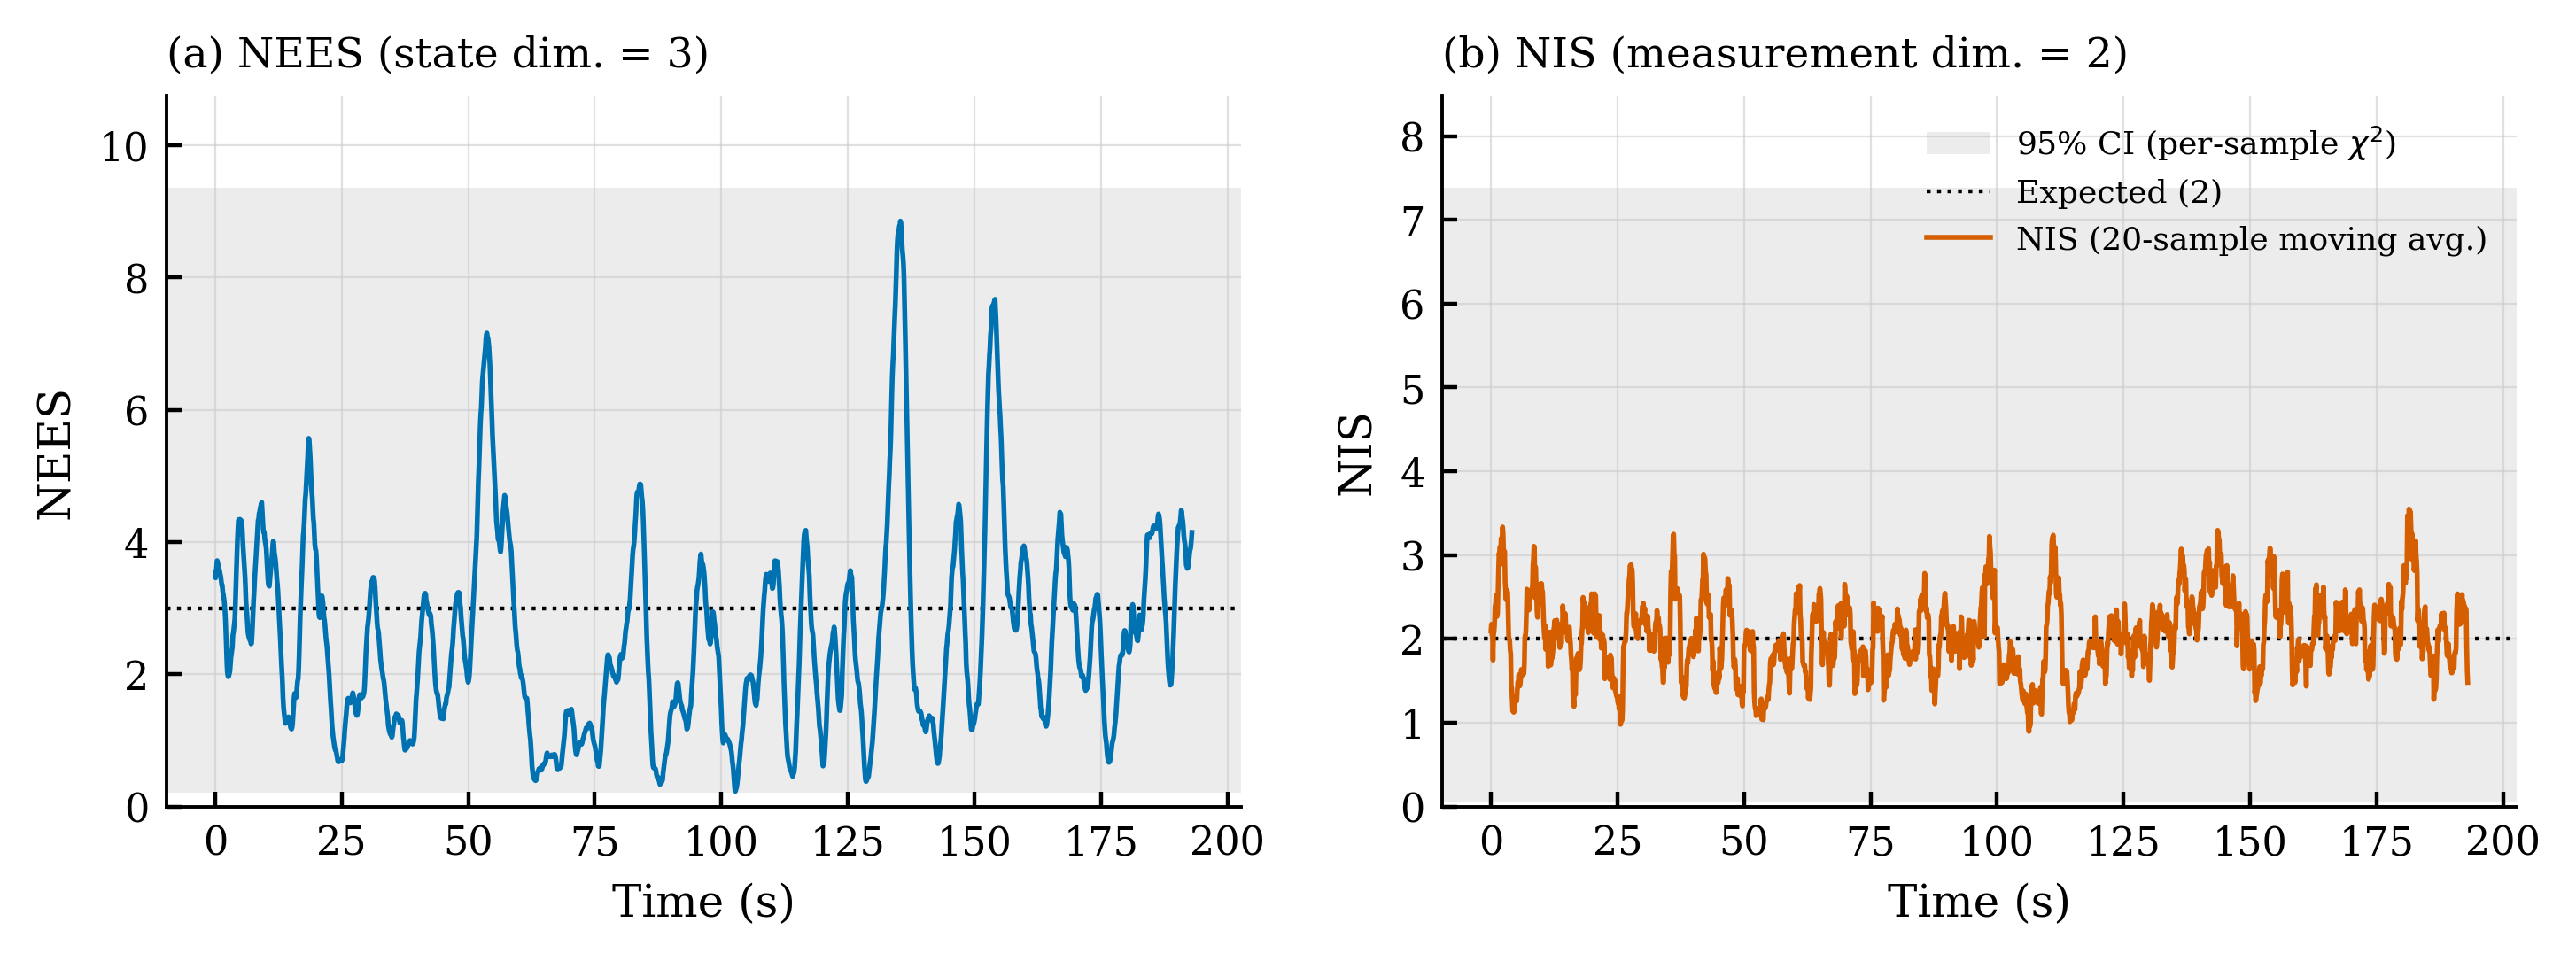
\includegraphics[width=0.85\textwidth]{../lafusion/figures/lafusion_nees_nis.png}

\vspace{0.2cm}
\small NEES e NIS ao longo dos 2000 passos da validação Monte Carlo (30 sementes), com valores esperados teóricos (3,0 e 2,0) e faixa de confiança 95\%.

\vspace{0.15cm}
\small \emph{Por que esta figura importa:} a tabela do slide anterior mostra só a média agregada das 30 sementes — não mostra \textbf{se} o filtro permanece consistente ao longo de toda a trajetória ou só na média. Esta figura confirma que NEES/NIS oscilam em torno do valor esperado de forma estável do início ao fim da corrida, não só nos primeiros ou últimos passos — evidência de que a calibração do filtro (Q, R) não depende de um regime transitório específico antes de ser aplicada aos dados reais.
\end{frame}

% ============================================================
\begin{frame}{LAFusion — Resultado principal}
\begin{table}
\small
\begin{tabular}{lcccc}
\toprule
\textbf{Regime de drift} & \textbf{Média EKF/Odom} & \textbf{$\Delta$ média} & \textbf{RMSE EKF/Odom} & \textbf{$\Delta$ RMSE} \\
\midrule
Nenhum (odom = GT) & 0,036 / 0,000 & N/A & 0,052 / 0,000 & N/A \\
Leve & 0,053 / 0,050 & $-5,3\%$ & 0,068 / 0,066 & $-2,1\%$ \\
Agressivo & 0,128 / 0,168 & \textbf{+23,7\%} & 0,163 / 0,195 & \textbf{+16,7\%} \\
\bottomrule
\end{tabular}
\caption{\small Erro de posição (m) nos instantes de correção YOLO, agregado em 3 cenários ($n=1323$). Wilcoxon $p<0{,}001$ sob drift agressivo.}
\end{table}

Sob drift agressivo, o EKF reduz o erro médio em \textbf{+23,7\%} frente à odometria pura.

\vspace{0.2cm}
\small \emph{Por quê o ganho é negativo sob drift leve ($-5{,}3\%$):} o erro de detecção visual ($\approx$3–6 cm) ainda não é menor que o erro de odometria pouco corrompida nesse regime — fundir as duas não ajuda, e pode piorar levemente. É comportamento esperado de um filtro corretamente calibrado, não uma falha.
\end{frame}

% ============================================================
\begin{frame}{LAFusion — Trajetória estimada}
\centering
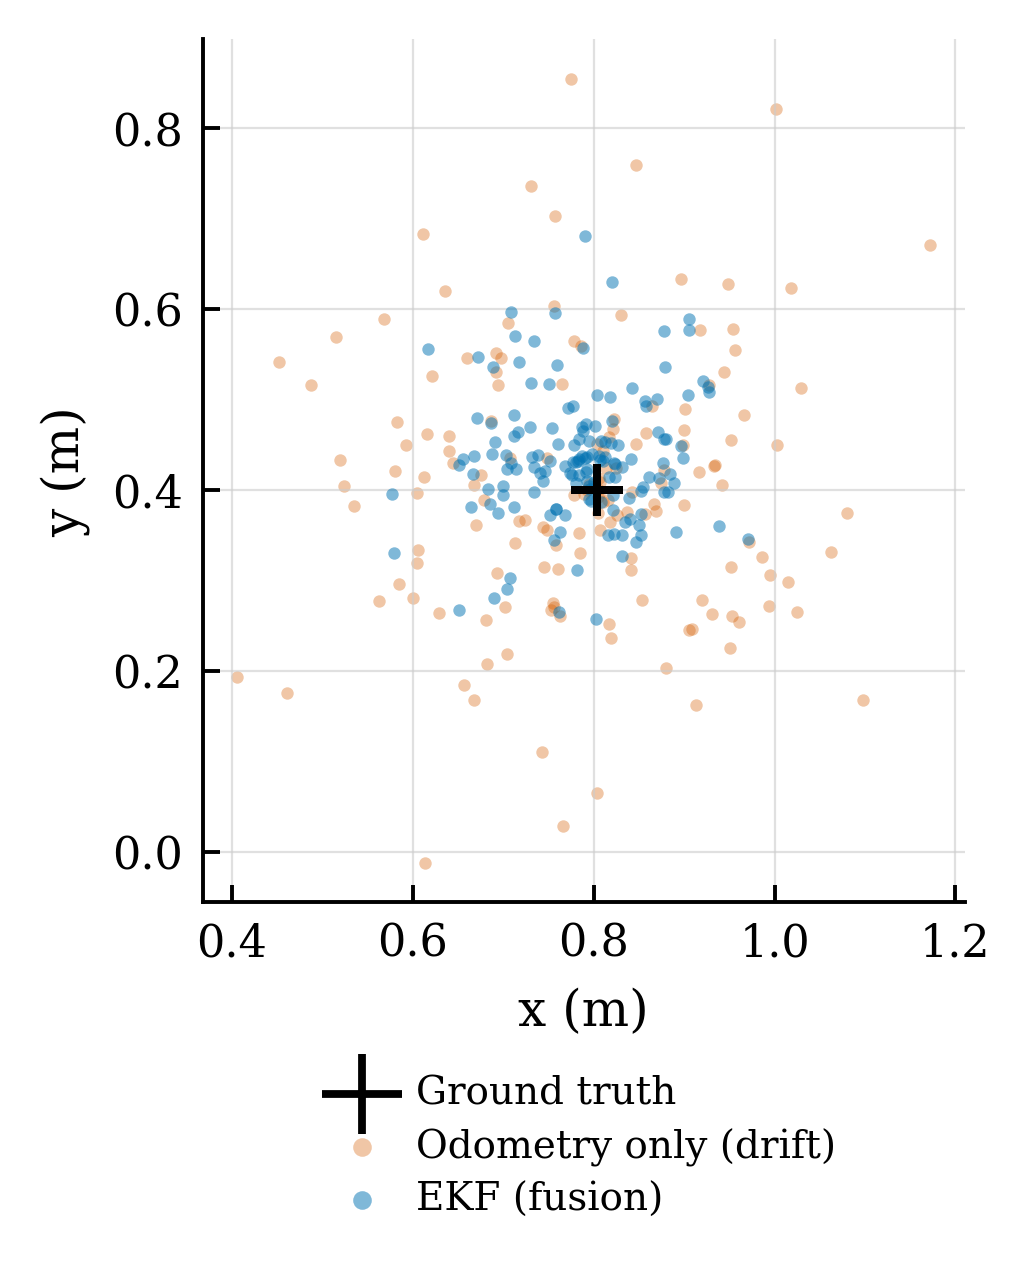
\includegraphics[width=0.62\textwidth]{../lafusion/figures/lafusion_trajectory.png}

\vspace{0.2cm}
\small Cenário 2 (movimento reto) sob drift agressivo: EKF (azul) vs. odometria bruta com drift (laranja, tracejada) vs. verdade terrestre (preto).

\vspace{0.15cm}
\small \emph{Por que esta figura importa:} a tabela anterior reduz o ganho de +23,7\% a um único número agregado — esta figura mostra \textbf{o mecanismo} por trás dele: a odometria bruta visivelmente se afasta do caminho reto real, enquanto a estimativa do EKF permanece próxima da trajetória verdadeira. É a evidência qualitativa de que o filtro está corrigindo o drift, não só de que uma métrica agregada melhorou.
\end{frame}

% ============================================================
\begin{frame}{LAFusion — Achado central: o erro contínuo}
\begin{table}
\scriptsize
\begin{tabular}{lccccc}
\toprule
\textbf{Cenário} & \textbf{Cobertura} & \textbf{Média EKF/Odom} & \textbf{$\Delta$} & \textbf{RMSE EKF/Odom} & \textbf{$\Delta$ RMSE} \\
\midrule
Parado & 27,6\% & 0,212 / 0,177 & $-19,3\%$ & 0,246 / 0,205 & $-19,8\%$ \\
Reto & 11,3\% & 0,212 / 0,178 & $-18,8\%$ & 0,245 / 0,206 & $-19,2\%$ \\
Curva/oclusão & 0,0\% & 0,178 / 0,178 & $-0,0\%$ & 0,205 / 0,205 & $-0,0\%$ \\
\textbf{Agregado} & --- & \textbf{0,200 / 0,178} & \textbf{$-12{,}7\%$} & \textbf{0,233 / 0,205} & \textbf{$-13{,}4\%$} \\
\bottomrule
\end{tabular}
\caption{\small Erro medido a CADA leitura de odometria, não só nos instantes de correção ($n=1607$, Wilcoxon $p<0{,}001$).}
\end{table}

Medido continuamente, o mesmo filtro é \textbf{12,7\% pior} que odometria pura — sinal invertido em relação ao slide anterior. No cenário de 0\% de cobertura, a mudança é exatamente 0,0\%: sem correções, a predição do EKF degenera matematicamente para integração pura de delta-odometria, idêntica à baseline não fundida — confirmação, não coincidência.

\vspace{0.2cm}
\small \textbf{Isso não invalida a contribuição:} reportar as duas métricas — em vez de só a favorável — é o ponto do trabalho, não uma admissão de fracasso.
\end{frame}

% ============================================================
\begin{frame}{LAFusion — Por que o erro contínuo piora (fundamentação teórica)}
\begin{columns}[T]
\begin{column}{0.42\textwidth}
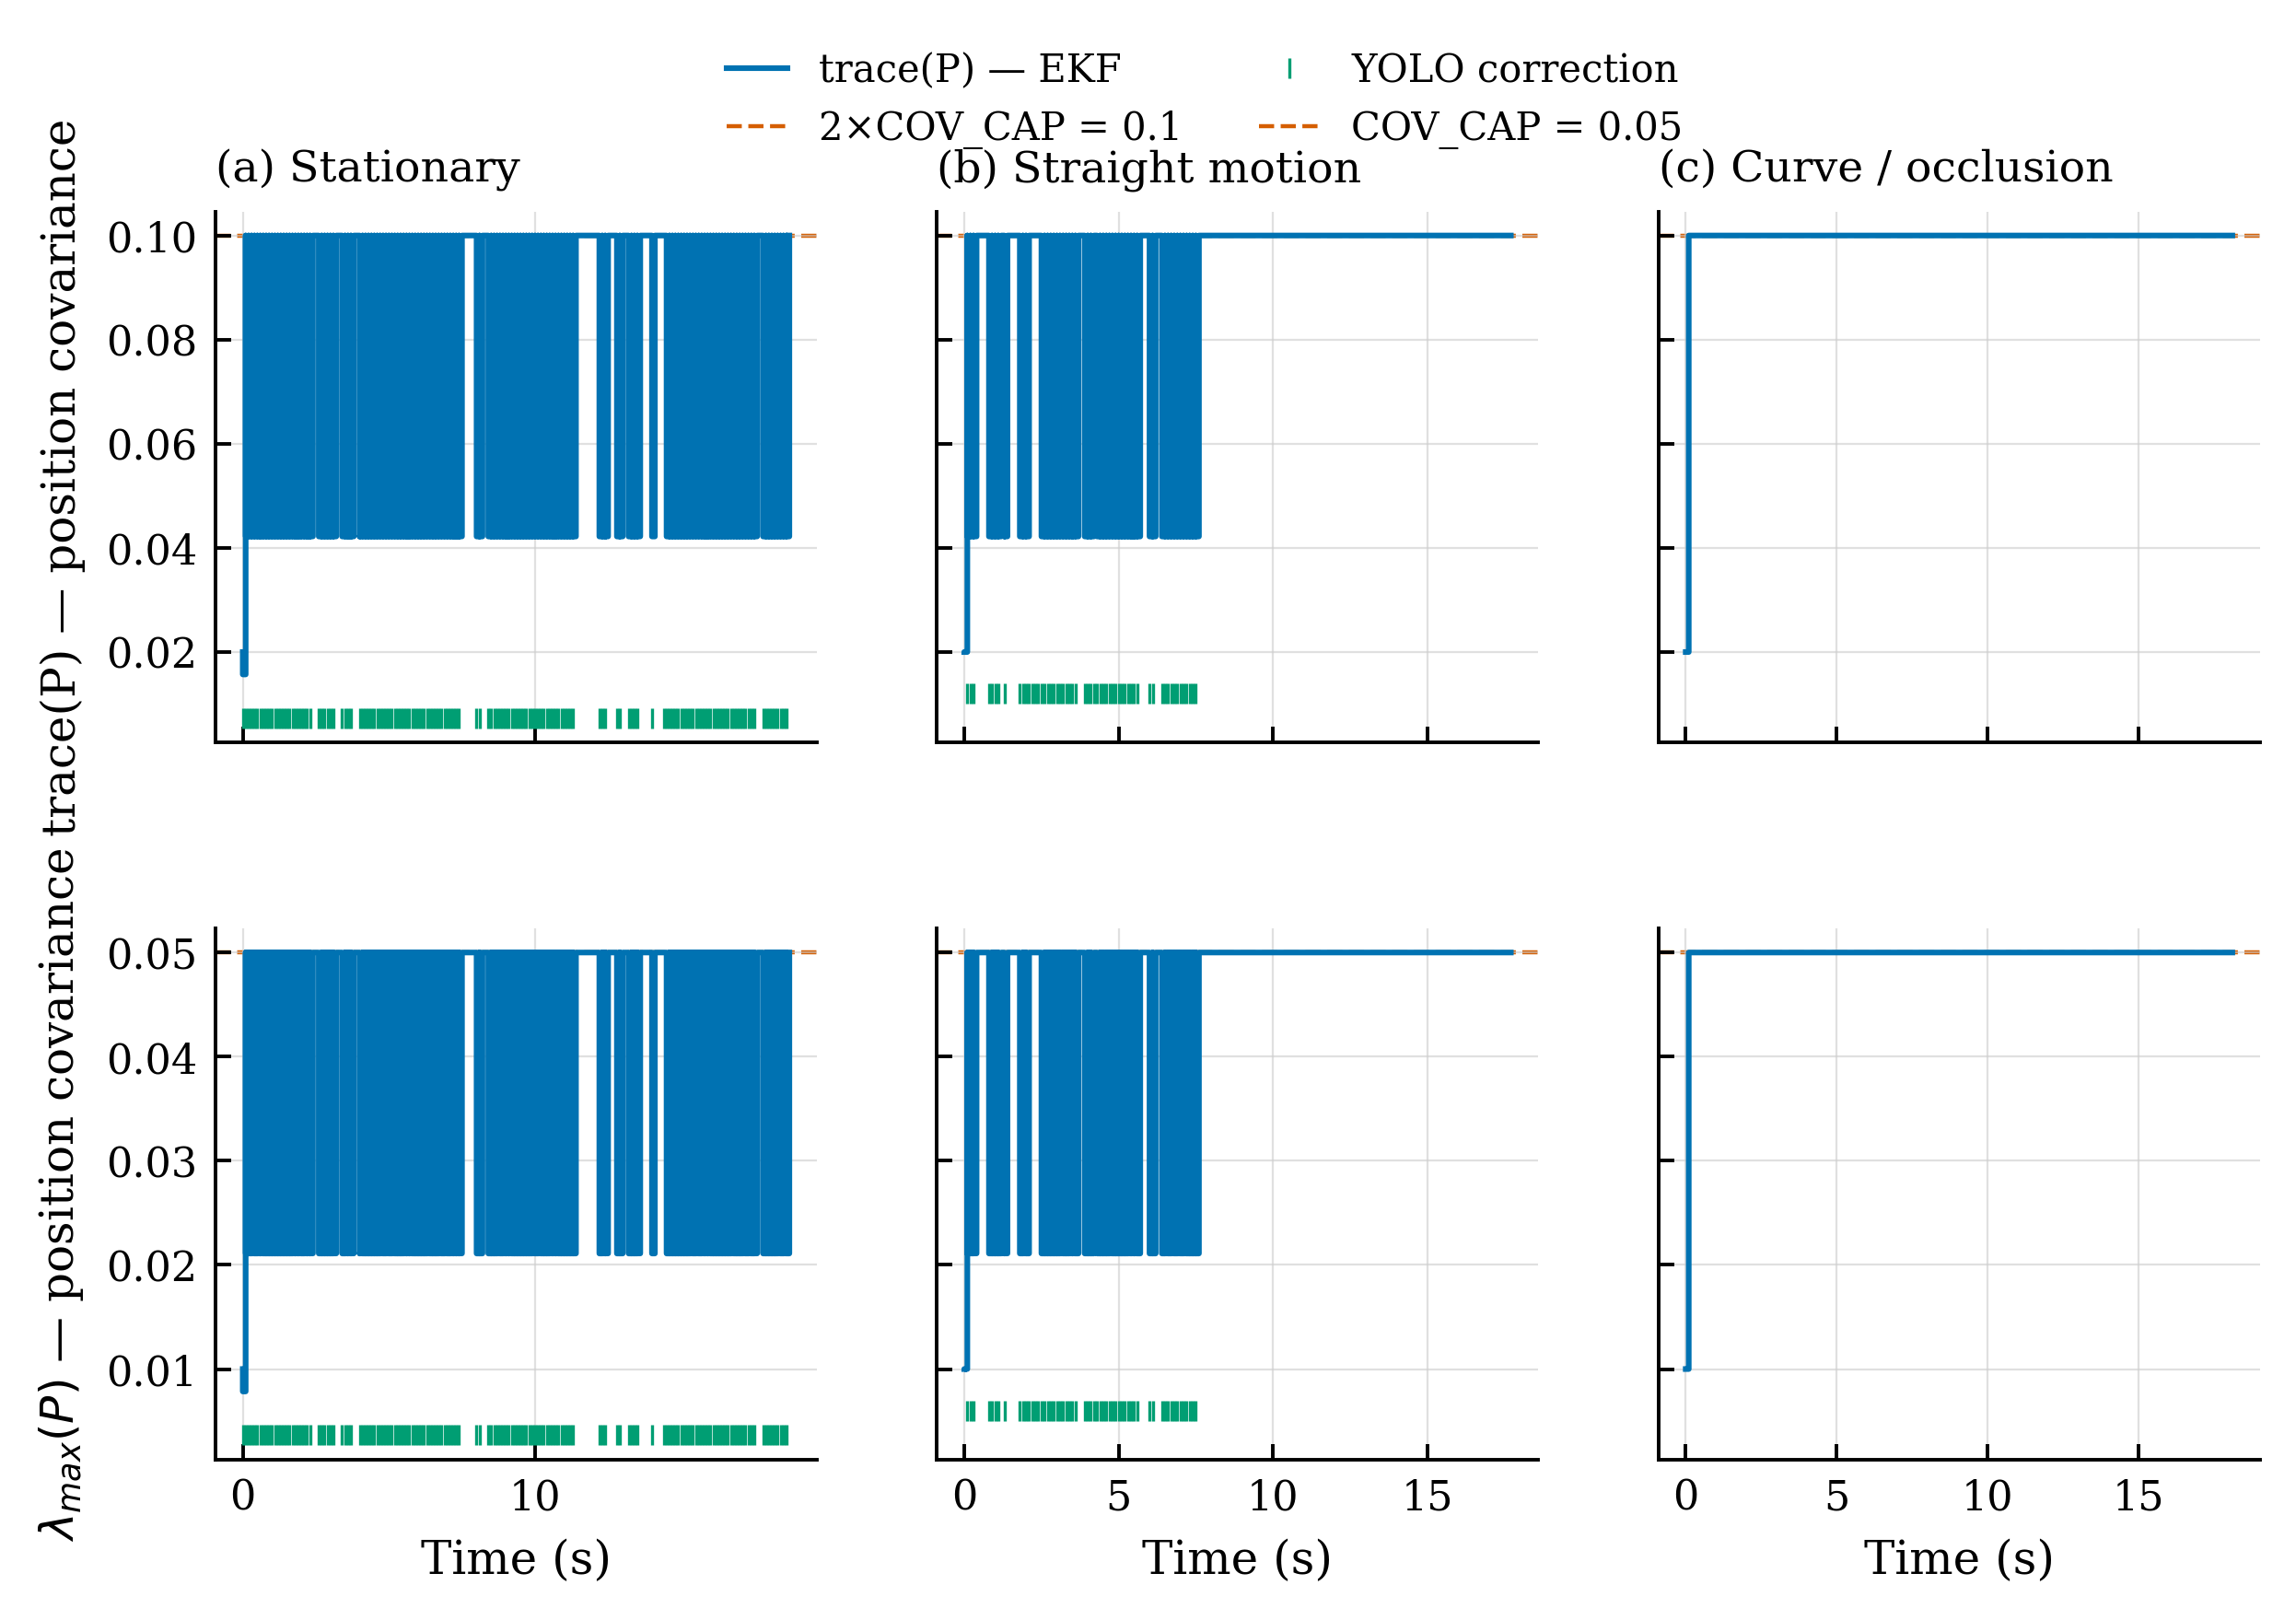
\includegraphics[width=\textwidth]{../lafusion/figures/lafusion_covariance_trace.png}
\end{column}
\begin{column}{0.58\textwidth}
\scriptsize
A covariância satura no teto quase imediatamente após qualquer intervalo sem correção (Sinopoli et al. 2004: divergência de covariância abaixo de uma taxa crítica de observação — nosso cenário de 0\% de cobertura está no caso-limite $p\to0$). O teto evita crescimento ilimitado, mas capa a \emph{estimativa de incerteza do próprio filtro}, não torna a estimativa de estado mais precisa — o filtro fica excessivamente confiante na predição só-odometria. Dissanayake et al. (2001) provam convergência do EKF-SLAM sob observação \emph{densa}; nossa câmera viola essa premissa por construção (0–28\% de cobertura).

\vspace{0.2cm}
\textbf{Por que UKF/partículas/IMM não resolvem:} um filtro de partículas degenera para propagação pura sem verossimilhança para reponderar; um UKF mira não-linearidade do modelo de observação, não a taxa de observação; um IMM ainda precisa de alguma observação para ponderar modos concorrentes. A causa raiz é a topologia do sensor (viewpoint único sujeito a oclusão), não a escolha do filtro.
\end{column}
\end{columns}
\end{frame}

% ============================================================
\begin{frame}{LAFusion — Estado atual: correção da calibração de câmera}
\small
\textbf{Achado desta sessão (16/08):} a calibração original, com os 4 intrínsecos livres ($f_x,f_y,c_x,c_y$), estava mal-condicionada — $f_x$ 33\% acima do valor geometricamente esperado, apesar de erro de reprojeção baixo (0,162px).

\vspace{0.15cm}
\scriptsize \emph{Causa raiz:} com a câmera fixa olhando reto para baixo, o tabuleiro de calibração fica sempre fronto-paralelo ao sensor em todas as poses — o caso degenerado clássico do método de Zhang (2000): sem variação de inclinação relativa entre sensor e alvo, $f_x$ e a distância percebida ficam quase linearmente dependentes.

\vspace{0.2cm}
\small\textbf{Correção aplicada:} como a geometria da câmera simulada já era conhecida com precisão (altura e campo de visão nominais exatos), fixamos $f_x,f_y,c_x,c_y$ no valor geométrico nominal e calibramos apenas a distorção — o remédio padrão quando os intrínsecos nominais já são confiáveis.

\vspace{0.2cm}
\textbf{Resultado:} a calibração corrigida reproduz a projeção heurística já usada em produção a menos de 0,001m de diferença — confirmando equivalência geométrica. \textbf{Nenhum resultado já publicado no paper muda}: a heurística de produção nunca esteve errada, só uma calibração alternativa em teste estava mal-condicionada.

\vspace{0.2cm}
\textbf{Estado:} paper com 8 páginas escritas (limite real do CFP é 12), prazo de submissão \textbf{04/09/2026}, formato Springer CCIS, revisão double-blind via Microsoft CMT.
\end{frame}

% ============================================================
\begin{frame}{Referências-chave e próximos passos}
\begin{columns}[T]
\begin{column}{0.5\textwidth}
\textbf{LARS — bibliografia essencial:}
\scriptsize
\begin{itemize}
\item Henderson et al. (2018) — reprodutibilidade em RL profundo, motiva o teste pareado usado aqui.
\item Huang \& Ontañón (2022) — action masking produz gradiente de política válido; nosso domínio difere do deles porque o masking elimina a violação sem fechar o gap.
\item Agrawal et al. (2023, RTAW) e Paul et al. (2022, Capsule Attention) — arquiteturas atencionais como direção futura.
\end{itemize}
\normalsize
\vspace{0.15cm}
\small\textbf{Próximos passos:} aguardar notificação de aceite (15/09/2026); espaço de ação e orçamento de treino maiores, guiados pelo diagnóstico causal; formulação Dec-POMDP (CTDE) como trabalho futuro.
\end{column}
\begin{column}{0.5\textwidth}
\textbf{LAFusion — bibliografia essencial:}
\scriptsize
\begin{itemize}
\item Sinopoli et al. (2004) e Censi (2009) — fundamentam por que o erro contínuo piora sob observação intermitente.
\item Bailey \& Durrant-Whyte (2006) — modelo EKF padrão que o filtro segue.
\item Dissanayake et al. (2001) — convergência sob observação densa, premissa violada por construção aqui.
\end{itemize}
\normalsize
\vspace{0.15cm}
\small\textbf{Próximos passos:} submissão no CMT até 04/09/2026; $Q$ adaptativo por tempo desde a última correção; LiDAR como terceira fonte de fusão (já publicado, não usado).
\end{column}
\end{columns}
\end{frame}

% ============================================================
\begin{frame}{Conclusão}
\textbf{LARS 2026:} um resultado negativo, testado e explicado causalmente — o PPO não supera a heurística gulosa neste cenário, e o \emph{action masking} refuta a explicação mais plausível a priori, redirecionando o diagnóstico para o espaço de ação pequeno e o orçamento de treino. A contribuição é a caracterização causal, não uma vitória do método proposto.

\vspace{0.4cm}
\textbf{LAFusion 2026:} um EKF de fusão sensorial entrega ganho real nos instantes de correção (+23,7\%), mas é mensuravelmente pior que odometria pura quando avaliado continuamente ($-$12,7\%) sob a cobertura visual esparsa que uma câmera fixa realmente produz — reversão explicada pela teoria estabelecida de filtragem de Kalman sob observação intermitente, não uma falha de implementação.

\vspace{0.4cm}
\centering \small Os dois trabalhos compartilham o mesmo padrão: reportar o resultado completo, favorável ou não, e fundamentá-lo — não filtrar para a métrica mais favorável.
\end{frame}

\end{document}
